\documentclass[11pt, a4paper]{article}
\usepackage[a4paper,
left=15mm,
right=15mm,
top=20mm,
bottom = 20mm]{geometry}
\usepackage{amsmath}
\usepackage{graphicx}
\usepackage{algorithm}
\usepackage{algorithmic}
\usepackage{multicol}
\usepackage{amsthm}
\usepackage{bm}
\usepackage{fancyhdr}

\usepackage{hyperref}
\hypersetup{
			hyperfootnotes=true,			
			bookmarks=true,			
			colorlinks=true,
			linkcolor=black,
                        linktoc=page,
			anchorcolor=black,
			citecolor=black,
			urlcolor=blue,
			pdftitle={LABAP},
			pdfkeywords={lapab, sapienza, roma, university}
}

\usepackage[table,xcdraw]{xcolor}

\def\arraystretch{1.5}

\begin{document}

\begin{titlepage}
	\begin{center}
		\vspace*{1cm}
		
		\Huge
		\textbf{LABAP Project - MyPics}
		\vspace{1.5cm}
		
		\Large
		Authors:\\
		\textbf{Mauro Ficorella 1941639}\\
		\textbf{Martina Turbessi 1944497}\\
		\textbf{Valentina Sisti 1952657}\\
		\vspace{0.5cm}
		
		\vfill
		
		
\includegraphics[width=0.3\textwidth]{images/Logo.jpg}
		
		\vfill
		
		\vspace{0.8cm}
		
		\Large
	\end{center}
\end{titlepage}

\tableofcontents

% Initial idea --------------------------------------------------------------------

\newpage

\section{Initial idea}
Interactive dashboard to look for images uploaded by other users.

\subsection{System objectives}
\begin{itemize}
    \item Show the dashboard with most popular images and images uploaded by followed users
    \item Manage user authentication
    \item Show a page related to users’ profiles containing all the images uploaded by them
    \item Allow users to upload, search and see images
    \item Allow users to follow other users to easily access their user profile and images
\end{itemize}

\subsection{Distributed Software Application with Containerization}
\begin{itemize}
    \item \textbf{Front-end layer}:
    \begin{itemize}
     \item Login/registration page
     \item Homepage
     \item User profile page
     \item User settings page
     \item Image visualization page with description and comments
     \item Image upload page
    \end{itemize}
    \item \textbf{API gateway}: to take an application user's request, route it to one or more backend services, gather the appropriate data and deliver it to the user in a single, combined package    
    \item \textbf{Logic layer}: 
    \begin{itemize}
     \item Microservice for user management: handles registration/authentication/access to the user profile
     \item Microservice for notifications: allows the user to be notified about new likes or new comments on his images and new followers
     \item Microservice for images management: handles the upload and deletion of images
     \item Microservice for social part: allows the user to like/comment/save an image and follow another user
     \item Microservice for search: handles the search of an image or an user
    \end{itemize}
    \item \textbf{Persistence layer}: NoSQL database
\end{itemize}
Each element of this list represents a different Docker container of the system and all the containers are orchestrated using Docker Compose.

\subsection{Potential Users}
\begin{itemize}
    \item People interested in discovering images from people that they follow
    \item People interested in uploading and sharing images
\end{itemize}

\subsection{Use Cases}
\begin{itemize}
    \item User can register to the app
    \item User can login into the app
    \item User can search for an image 
    \item User can search for an user
    \item User can visualize the home page containing most popular images and the images published by followed users 
    \item User can upload an image
    \item User can save an image
    \item User can remove an uploaded image
    \item User can like an image
    \item User can comment an image
    \item User can get notified if another user likes one of its images
    \item User can get notified if another user leave a comment on one of its images
    \item User can get notified for a new follower
    \item User can follow/unfollow another user
    \item User can access its own profile to visualize his images and the ones that he saved from other users
    \item User can access its own profile to manage it
    \item User can access another user profile to view his details and his published images
    \item User can logout
    \item User can delete its account
\end{itemize}

% User stories and prototypes -----------------------------------------------------

\newpage

\section{User stories and mockups}

\subsection{Sign-up}
\begin{table}[H]
    \centering
    \begin{tabular}{|p{4cm}|p{4cm}|p{4cm}|p{4cm}|}
    \hline
    \rowcolor[HTML]{EFEFEF} 
    AS A  & I WANT TO              & SO THAT I CAN     & ADDED BY \\ \hline
    Guest & Register to the system & Create my profile & Everyone \\ \hline
    \end{tabular}
\end{table}
\begin{figure}[H]
    \centering
    \fbox{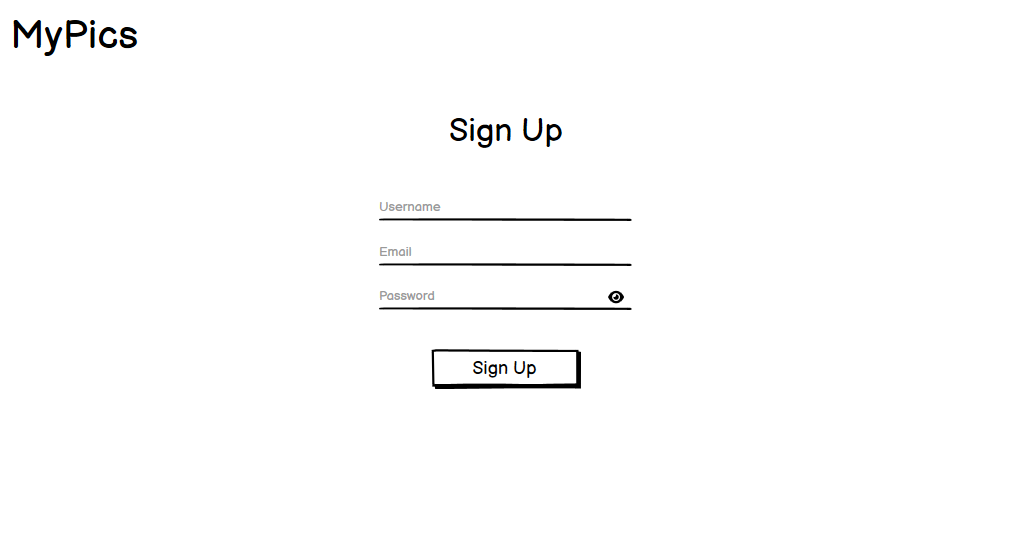
\includegraphics[width=0.67\textwidth]{images/sign-up.png}}
    %\caption{Caption}
    %\label{fig:my_label}
\end{figure}

\subsection{Login}
\begin{table}[H]
    \centering
    \begin{tabular}{|p{4.5cm}|p{4cm}|p{4cm}|p{4cm}|}
    \hline
    \rowcolor[HTML]{EFEFEF} 
    AS A                       & I WANT TO             & SO THAT I CAN         & ADDED BY \\ \hline
    Non-logged registered user & Login into the system & Use system's services & Everyone \\ \hline
    \end{tabular}
\end{table}
\begin{figure}[H]
    \centering
    \fbox{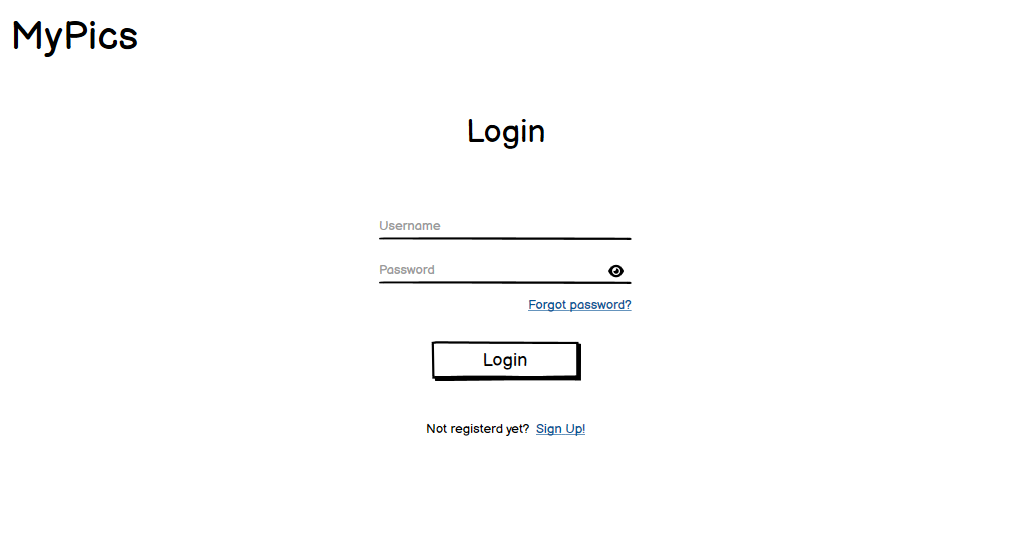
\includegraphics[width=0.7\textwidth]{images/login.png}}
    %\caption{Caption}
    %\label{fig:my_label}
\end{figure}

\subsection{User settings}
\begin{table}[H]
    \centering
    \begin{tabular}{|p{4cm}|p{4.5cm}|p{5cm}|p{3cm}|}
    \hline
    \rowcolor[HTML]{EFEFEF} 
    AS A                    & I WANT TO                      & SO THAT I CAN                     & ADDED BY \\ \hline
    Logged registered user  & Logout from the system         & Login as another user             & Everyone \\ \hline
    Logged user             & Delete my profile              & No longer access the system       & Everyone \\ \hline
    Logged user             & Access my profile settings     & Manage it                         & Everyone \\ \hline
    \end{tabular}
\end{table}
\begin{figure}[H]
    \centering
    \fbox{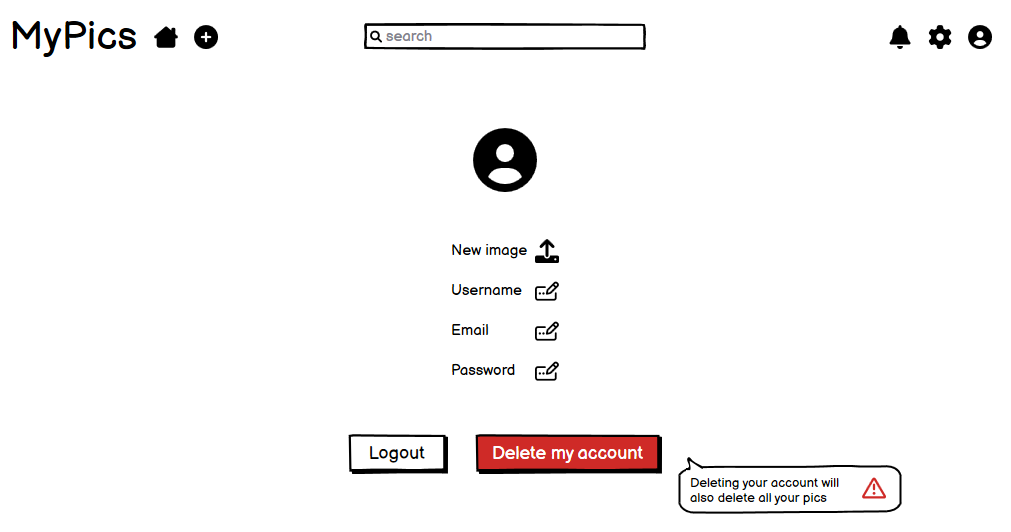
\includegraphics[width=0.6\textwidth]{images/settings.png}}
    %\caption{Caption}
    %\label{fig:my_label}
\end{figure}

\subsection{Main}
\begin{table}[H]
    \centering
    \begin{tabular}{|p{4cm}|p{4.5cm}|p{5cm}|p{3cm}|}
    \hline
    \rowcolor[HTML]{EFEFEF} 
    AS A        & I WANT TO                        & SO THAT I CAN                                  & ADDED BY \\ \hline
    Logged user & Access the homepage              & Discover the most popular images               & Everyone \\ \hline
    Logged user & Access the homepage              & Discover images published by followed users    & Everyone \\ \hline
    Logged user & Search for images                & Visualize them                                 & Everyone \\ \hline
    Logged user & Search for other users           & Visualize their profile and their images       & Everyone \\ \hline
    Logged user & Get notified                     & Know if another user liked or commented one of my image or followed me & Everyone \\ \hline
    Logged user & Access other user's profile page & Visualize his details and published images     & Everyone \\ \hline
    Logged user & Visualize image                  & Visualize its details and comments             & Everyone \\ \hline
    \end{tabular}
\end{table}
\begin{figure}[H]
    \centering
    \fbox{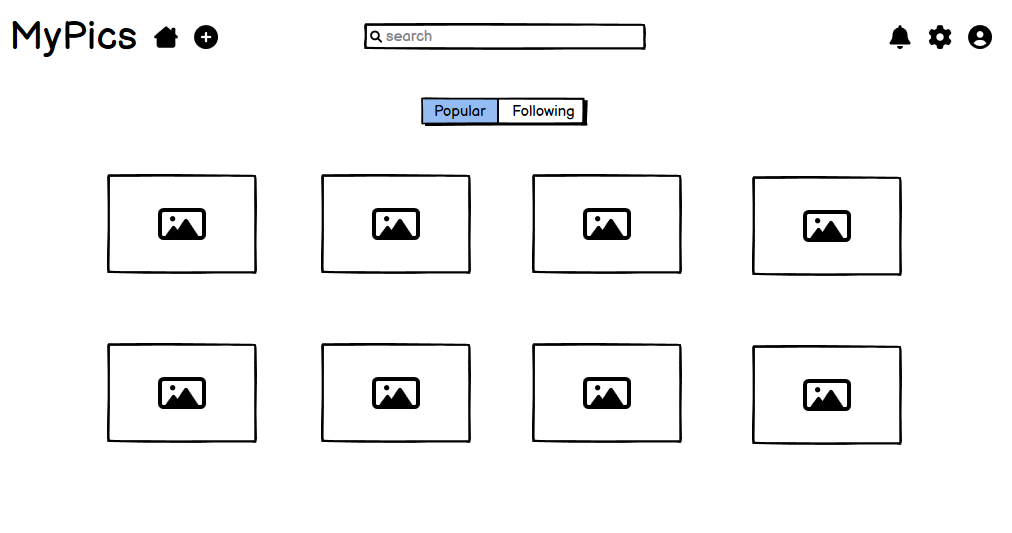
\includegraphics[width=0.7\textwidth]{images/home.png}}
    %\caption{Caption}
    %\label{fig:my_label}
\end{figure}

\subsection{Pic}
\begin{table}[H]
    \centering
    \begin{tabular}{|p{3.3cm}|p{4.5cm}|p{5.7cm}|p{3cm}|}
    \hline
    \rowcolor[HTML]{EFEFEF} 
    AS A        & I WANT TO                & SO THAT I CAN                       & ADDED BY \\ \hline
    Logged user & Like an image            & Express my appreciation about it    & Everyone \\ \hline
    Logged user & Save an image            & Discover the most popular images    & Everyone \\ \hline
    Logged user & Remove an uploaded image & Deny to other users to visualize it & Everyone \\ \hline    
    \end{tabular}
\end{table}
\begin{figure}[H]
    \centering
    \fbox{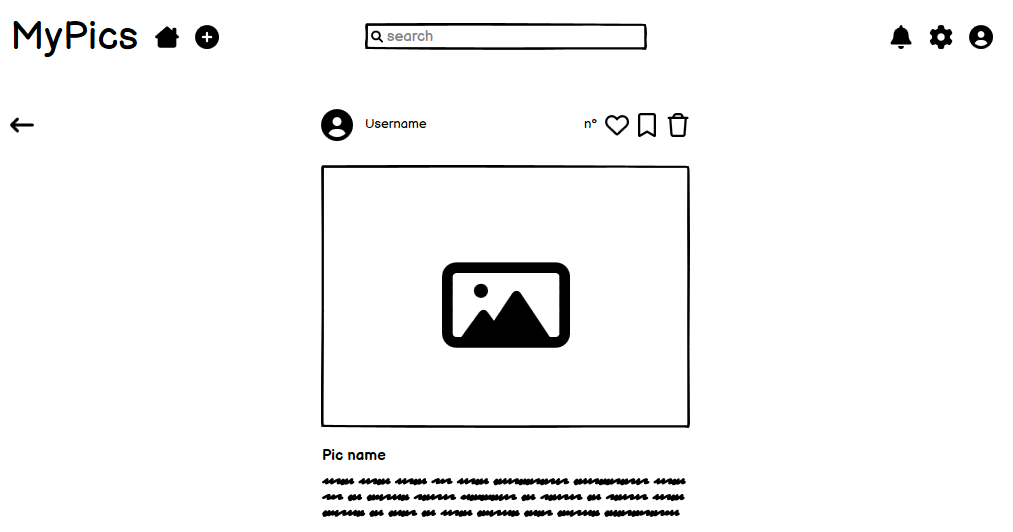
\includegraphics[width=0.7\textwidth]{images/pic.png}}
    %\caption{Caption}
    %\label{fig:my_label}
\end{figure}

\subsection{Upload pic}
\begin{table}[H]
    \centering
    \begin{tabular}{|p{4.5cm}|p{4cm}|p{5cm}|p{3cm}|}
    \hline
    \rowcolor[HTML]{EFEFEF} 
    AS A        & I WANT TO             & SO THAT I CAN                         & ADDED BY \\ \hline
    Logged user & Upload an image       & Share it with other users             & Everyone \\ \hline    
    \end{tabular}
\end{table}
\begin{figure}[H]
    \centering
    \fbox{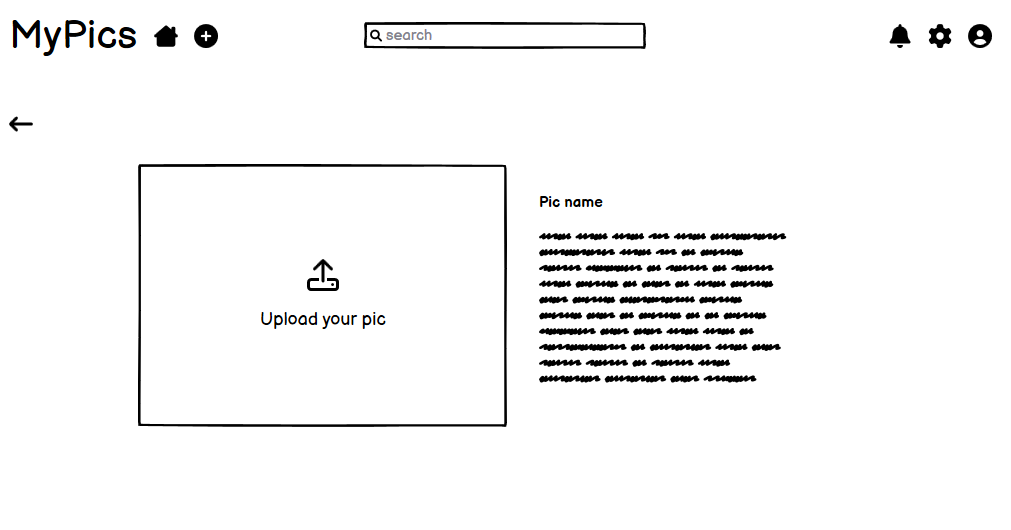
\includegraphics[width=0.6\textwidth]{images/addPic.png}}
    %\caption{Caption}
    %\label{fig:my_label}
\end{figure}

\subsection{User profile}
\begin{table}[H]
    \centering
    \begin{tabular}{|p{3.5cm}|p{4cm}|p{6cm}|p{3cm}|}
    \hline
    \rowcolor[HTML]{EFEFEF} 
    AS A        & I WANT TO             & SO THAT I CAN                         & ADDED BY \\ \hline
    Logged user & Access my profile     & Visualize all my published images     & Everyone \\ \hline 
    Logged user & Access my profile     & Visualize all my saved images         & Everyone \\ \hline 
    Logged user & Access user profile   & Visualize followers/followed users    & Everyone \\ \hline 
    Logged user & Follow another user   & Stay updated about his new images     & Everyone \\ \hline    
    \end{tabular}
\end{table}
\begin{figure}[H]
    \centering
    \fbox{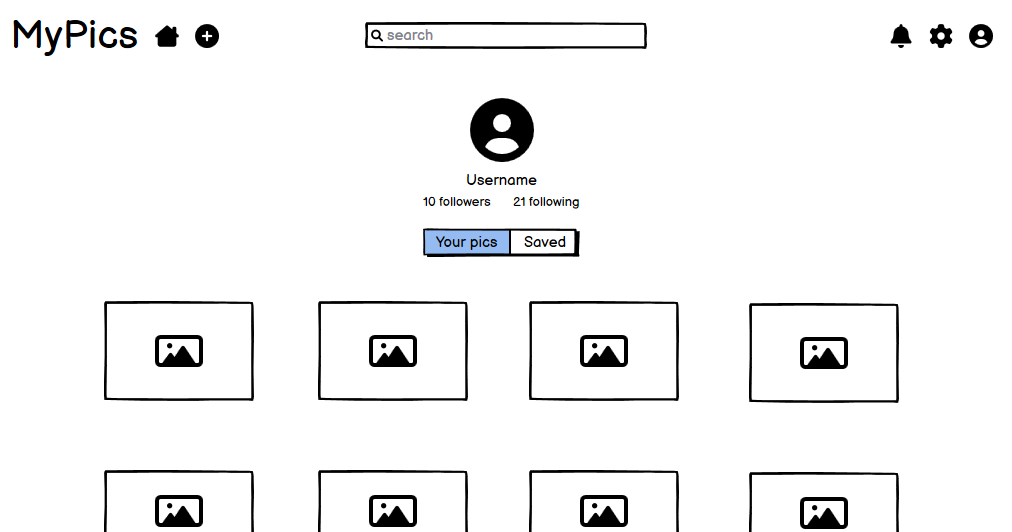
\includegraphics[width=0.7\textwidth]{images/profile.png}}
    \fbox{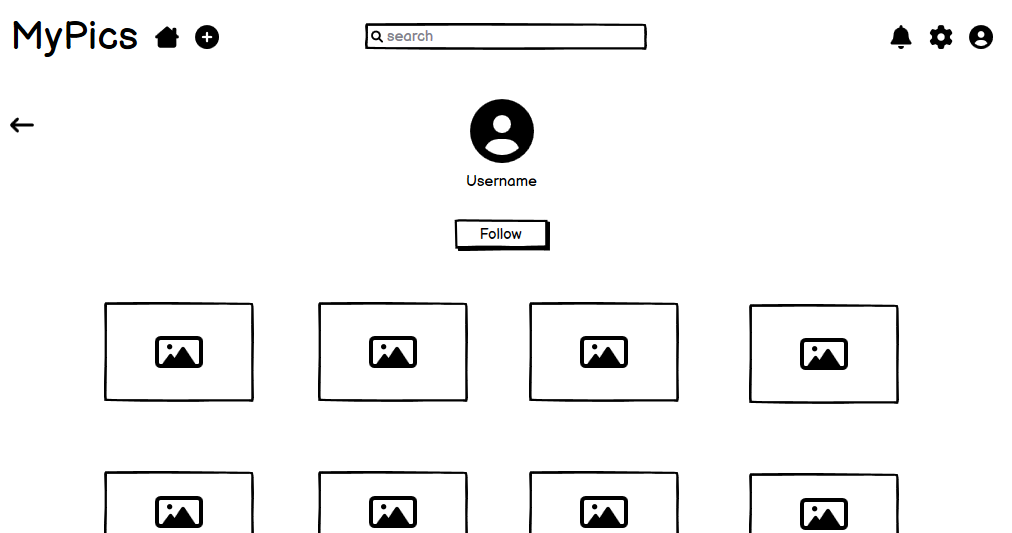
\includegraphics[width=0.7\textwidth]{images/user.png}}
    %\caption{Caption}
    %\label{fig:my_label}
\end{figure}

% Effort estimation ----------------------------------------------------------------

\newpage

\section{Effort estimation}

\subsection{Function Points} 
\begin{figure}[H]
    \centering
    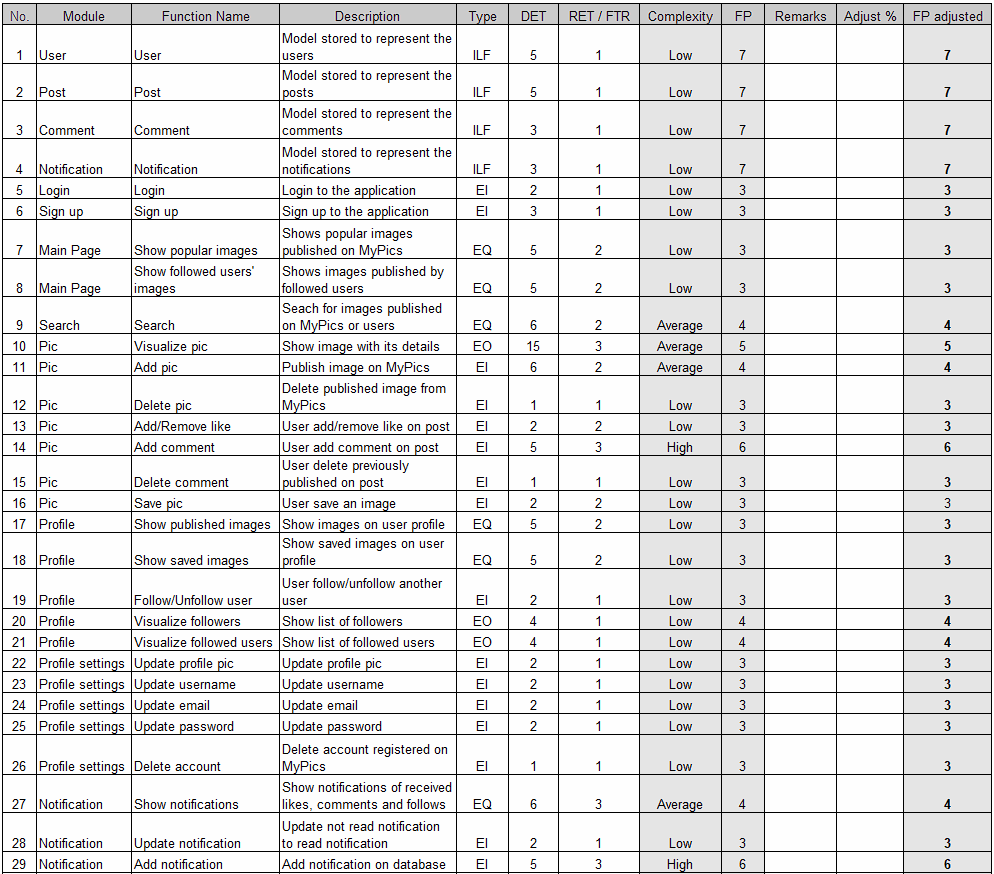
\includegraphics[width=1\textwidth]{images/FP.png}
\end{figure}
\begin{figure}[H]
    %\centering
    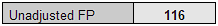
\includegraphics[width=0.25\textwidth]{images/UFP.png}
\end{figure}

\noindent
Considering Java as main language, this is equivalent to 6148 SLOC.

\newpage

\subsection{CoCoMo II} 
\begin{figure}[H]
    \centering
    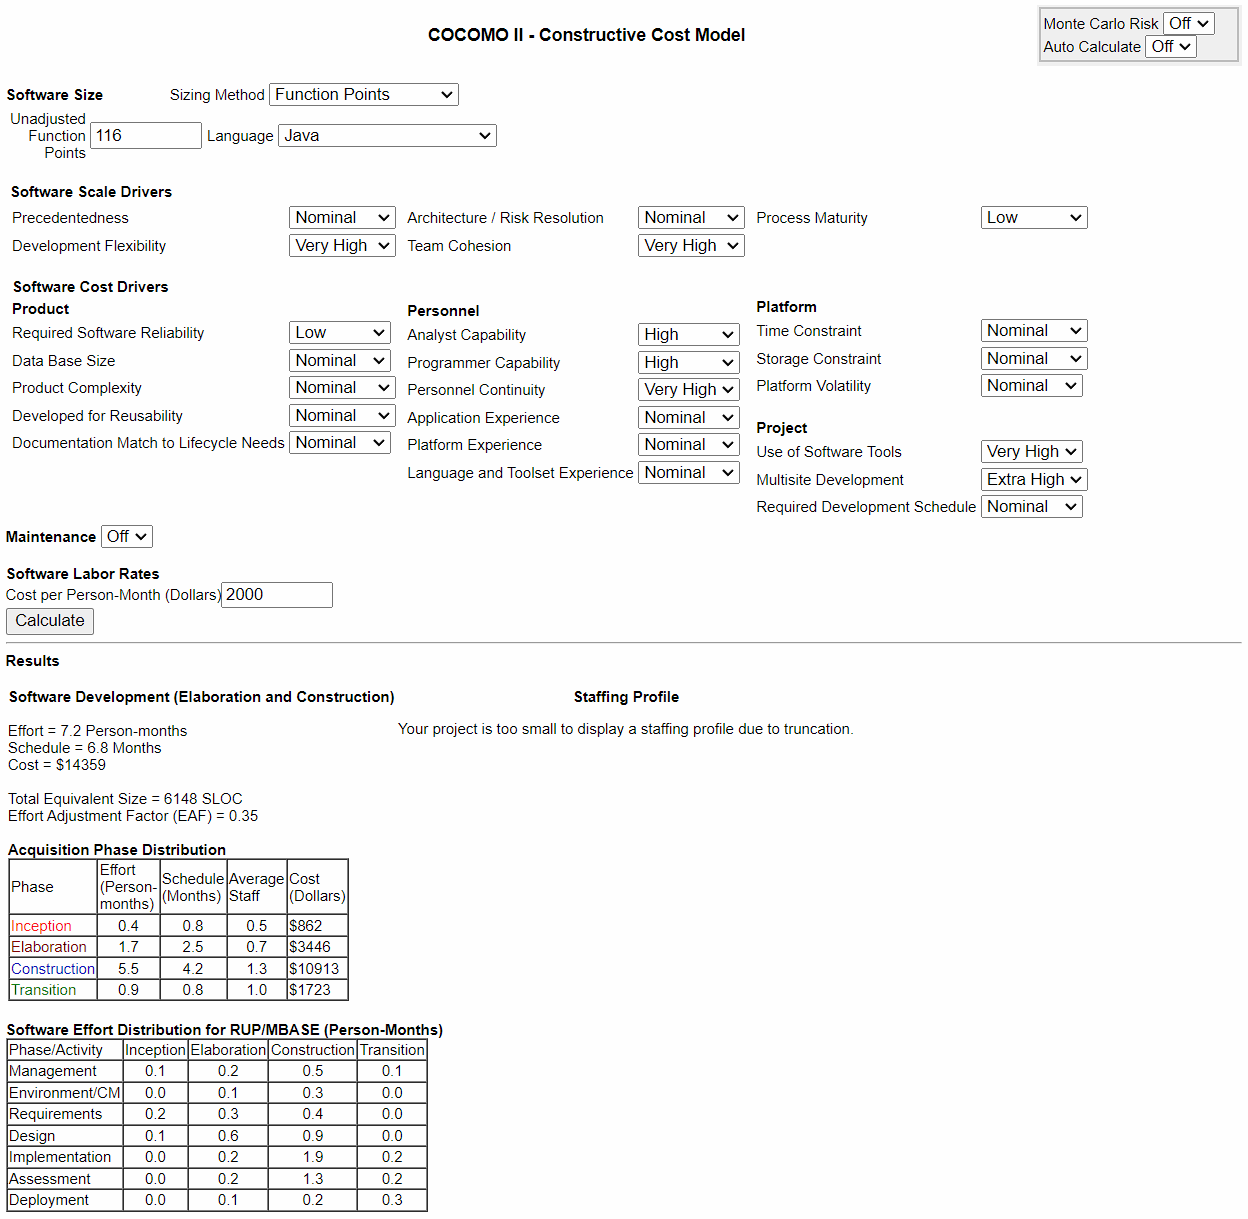
\includegraphics[width=1\textwidth]{images/cocomo.png}
\end{figure}

% System architecture ---------------------------------------------------------------

\newpage

\section{System architecture}
The system architecture is based on microservices, each running on its own Docker container and each accessing its own data. These containers are orchestrated through Docker Compose.
\begin{figure}[H]
    \centering
    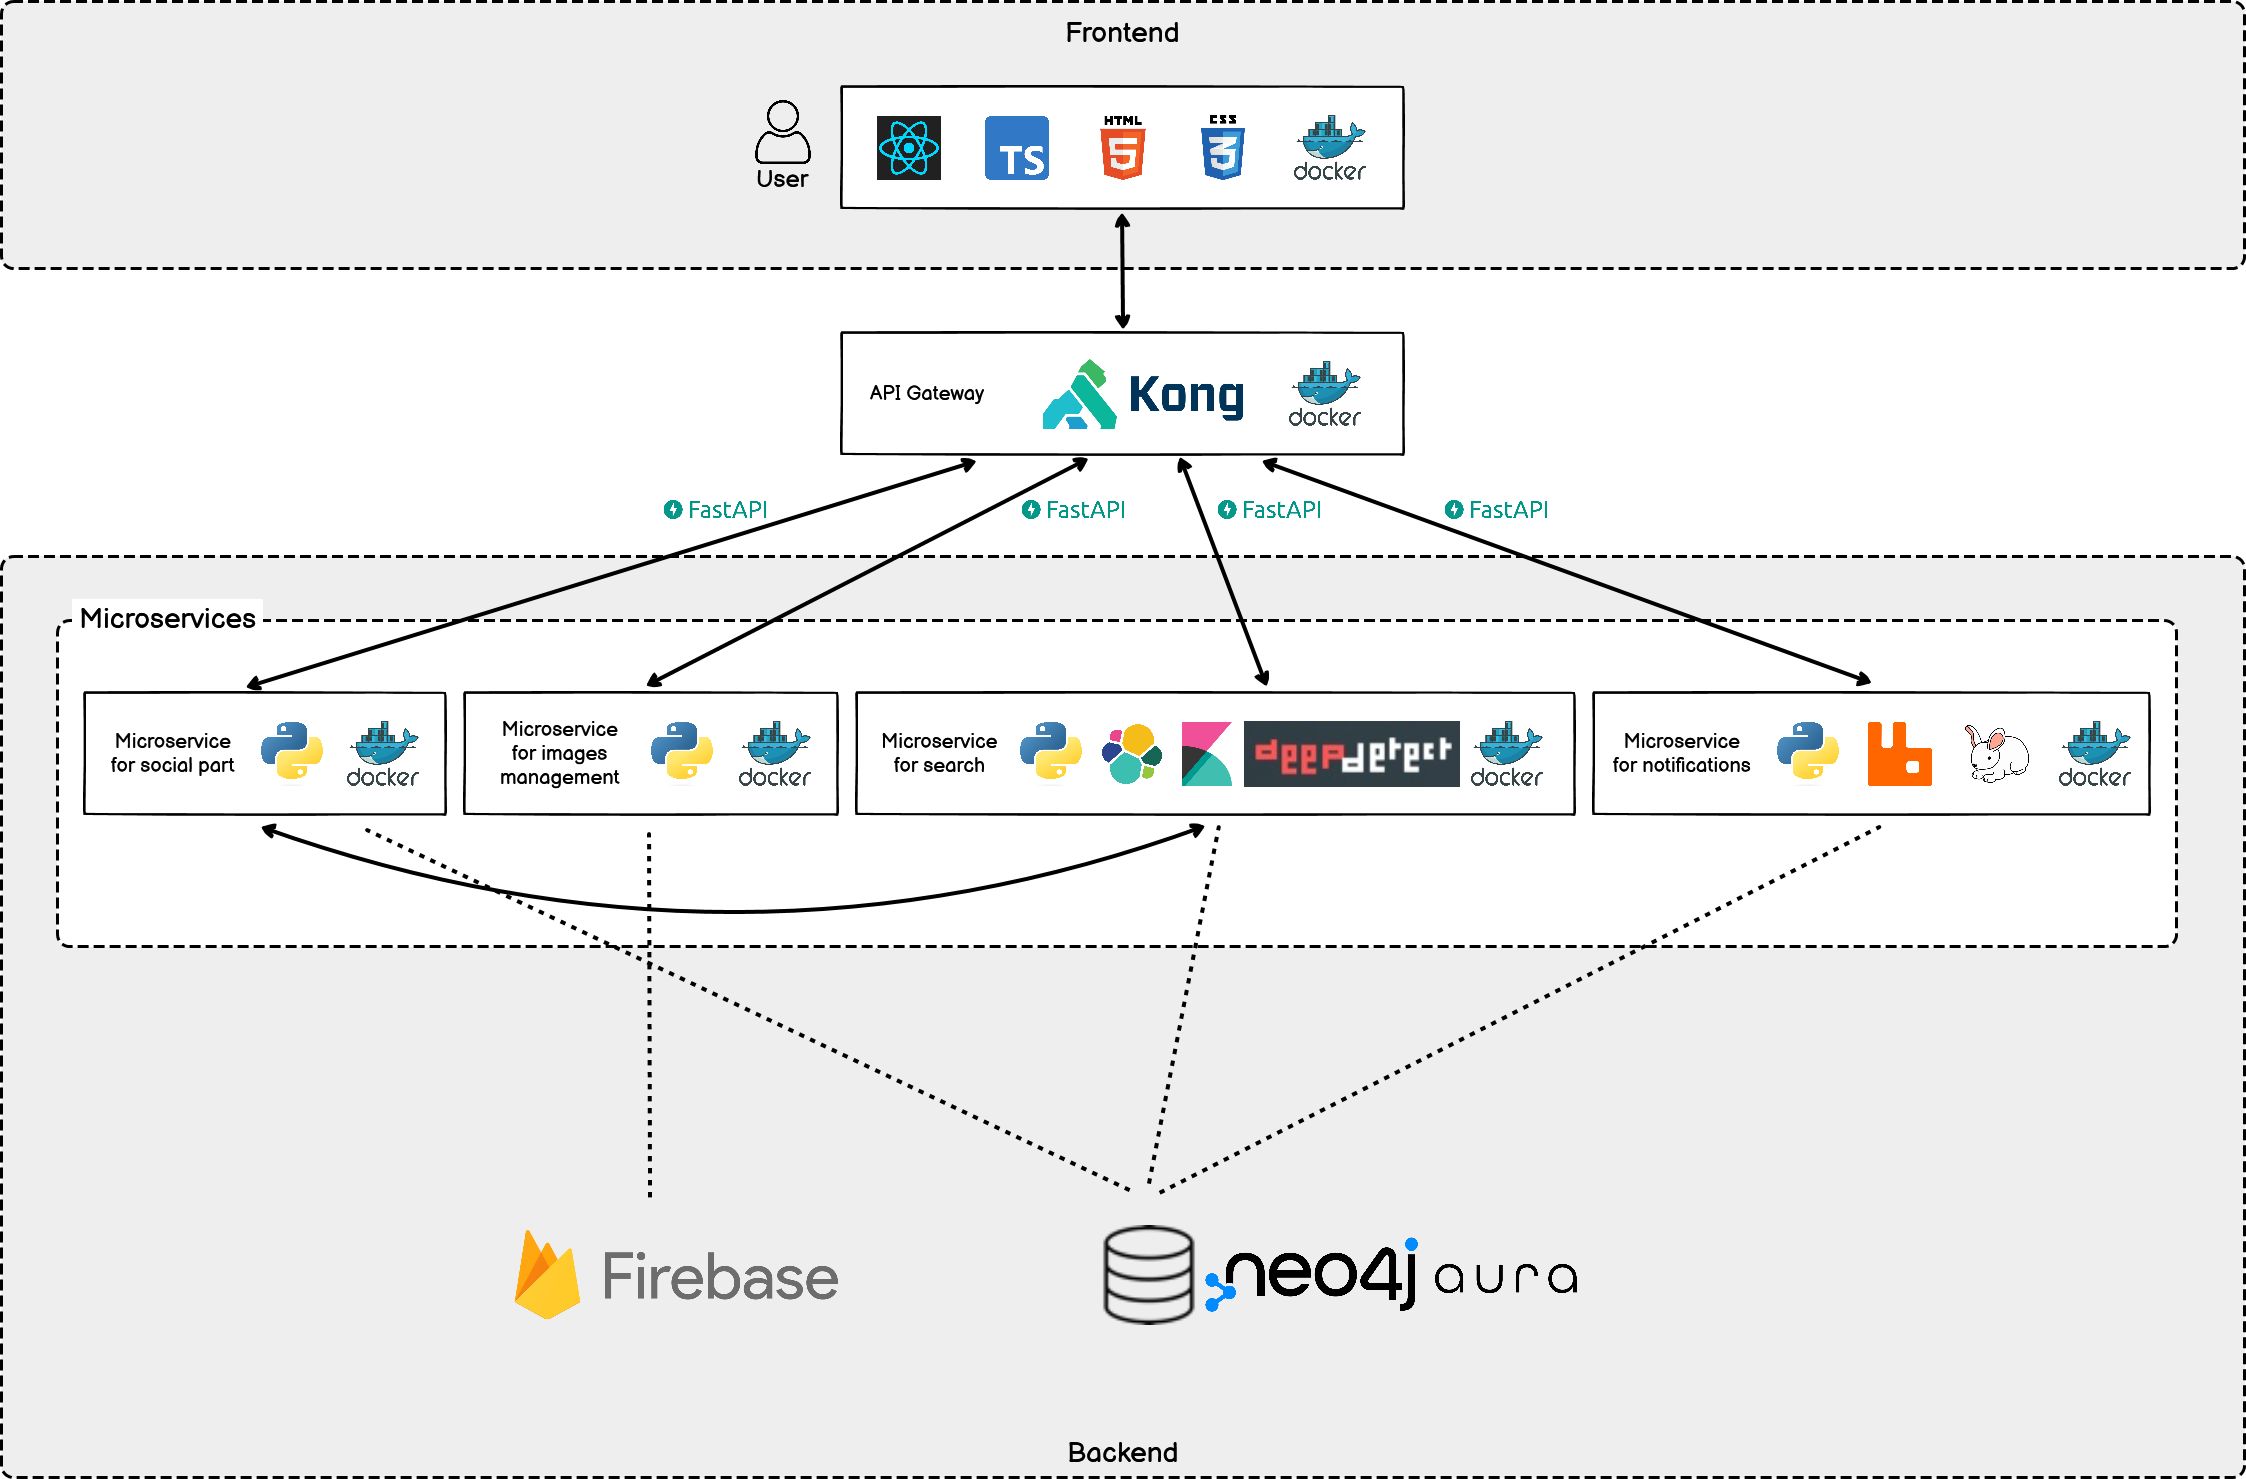
\includegraphics[width=1\textwidth]{images/architecture.png}
    \caption{Overview of system architecture}
\end{figure}
\begin{itemize}
    \item \textbf{Frontend:} developed in React (based on TypeScript, HTML and CSS). Users interact with the system through this layer.
    \item \textbf{API Gateway:} we use Kong Gateway which is a lightweight, fast, and flexible cloud-native API gateway that serves as a reverse proxy that lets us manage, configure, and route requests to our APIs exposed by the microservices.
    \item \textbf{Microservice for social part:} exposes APIs to manage all social aspects of the system (i.e. user registration, likes, comments, new posts).
    \item \textbf{Microservice for images management:} exposes APIs to upload images on the Firebase cloud storage.
    \item \textbf{Microservice for search:} we use Elasticsearch as search engine and Kibana, which provides search and data visualization capabilities for data indexed in Elasticsearch. Moreover we use Deepdetect deep learning platform which offers pre-trained models for classifing images' based on represented subjects and to be able to search for images based on them through Elasticsearch.
    \item \textbf{Microservice for notifications:} we use RabbitMQ message oriented middleware through CloudAMQP, which provides managed RabbitMQ servers in the cloud, in order to be able to access all the different queues in the cloud from any device.
    \item \textbf{Database:} we use Neo4j NoSQL graph database in order to store all the system data. In particular we use Neo4j AuraDB that offers a database instance in the cloud with which all the above mentioned microservices can communicate. 
\end{itemize}
We developed the backend microservices using Python and all of them expose a REST interface that leverages on FastAPI framework. 

% Sprint analytics --------------------------------------------------------------------

\newpage

\section{Sprint analytics}
Each sprint lasts 14 days (2 weeks).
\subsection{Sprint 1: 10/10/2022 - 21/10/2022}
\begin{figure}[H]
    \centering
    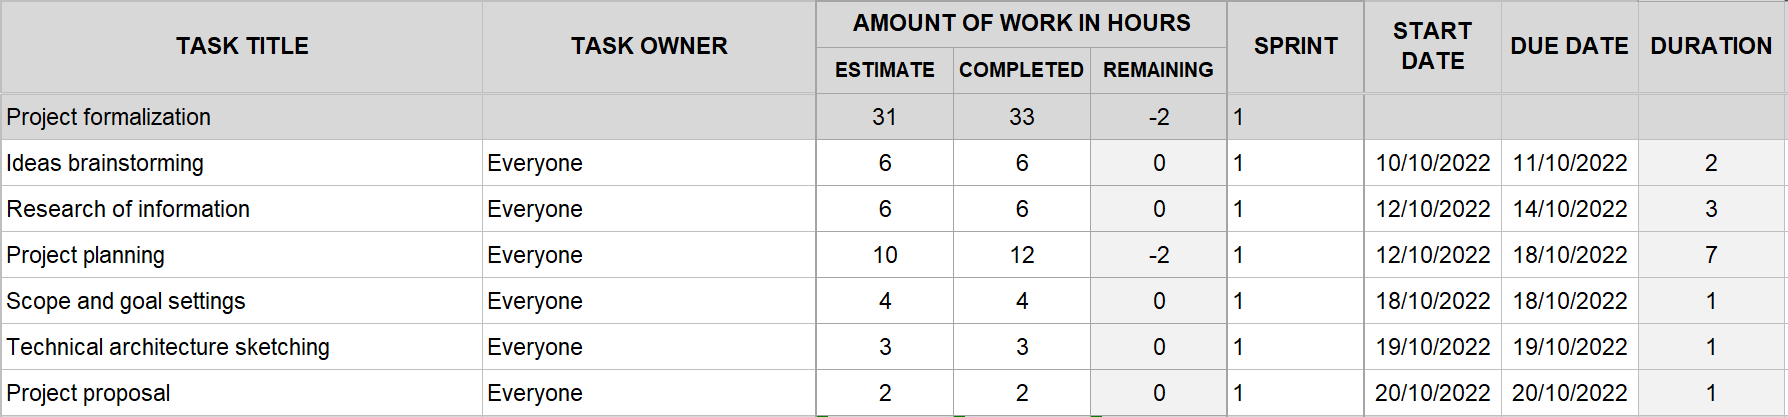
\includegraphics[width=1\textwidth]{images/sprint1.png}
\end{figure}
\subsection{Sprint 2: 06/02/2023 - 17/02/2023}
\begin{figure}[H]
    \centering
    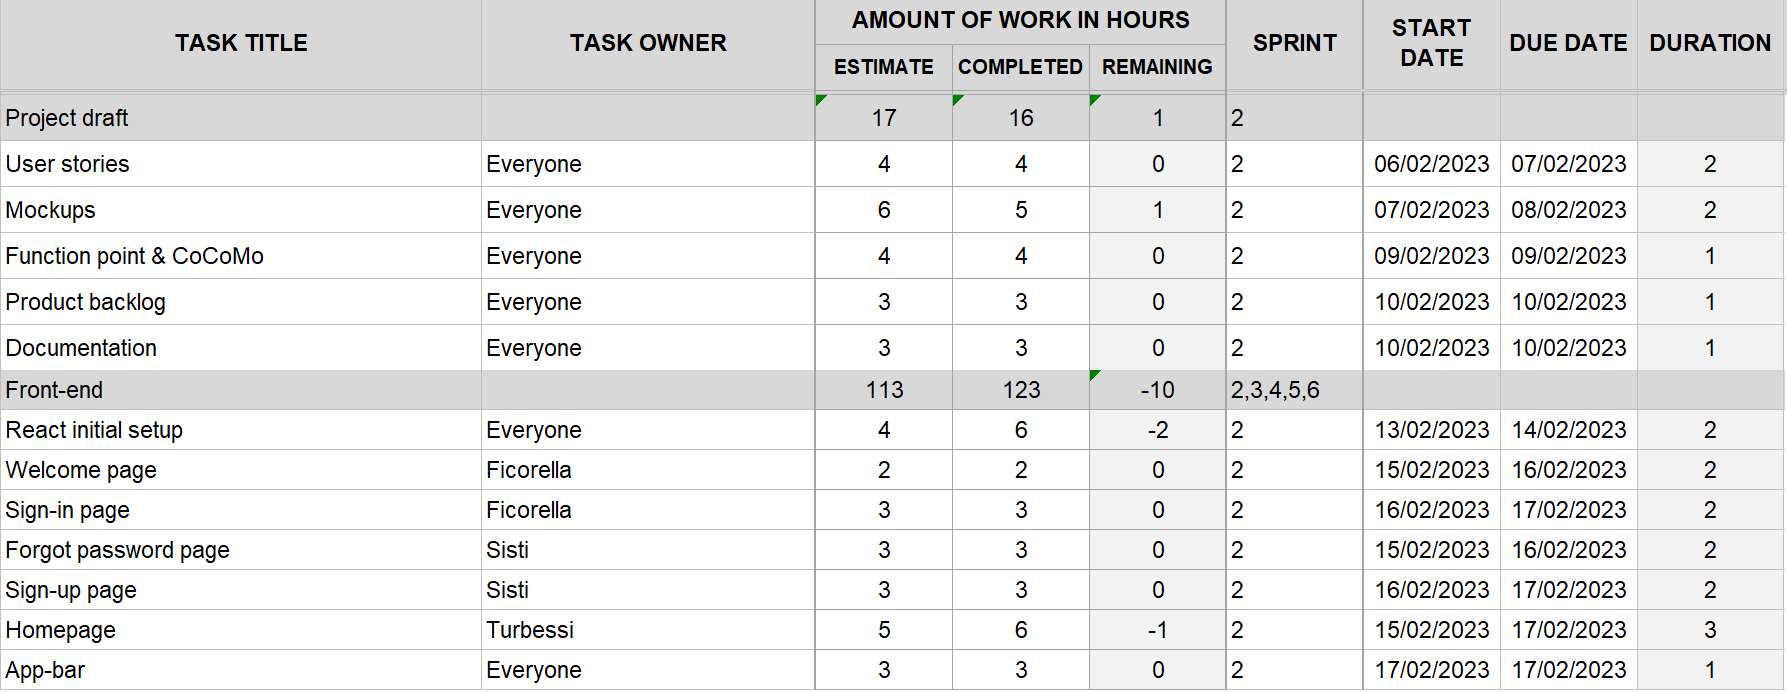
\includegraphics[width=1\textwidth]{images/sprint2.png}
\end{figure}
\subsection{Sprint 3: 20/02/2023 - 03/03/2023}
\begin{figure}[H]
    \centering
    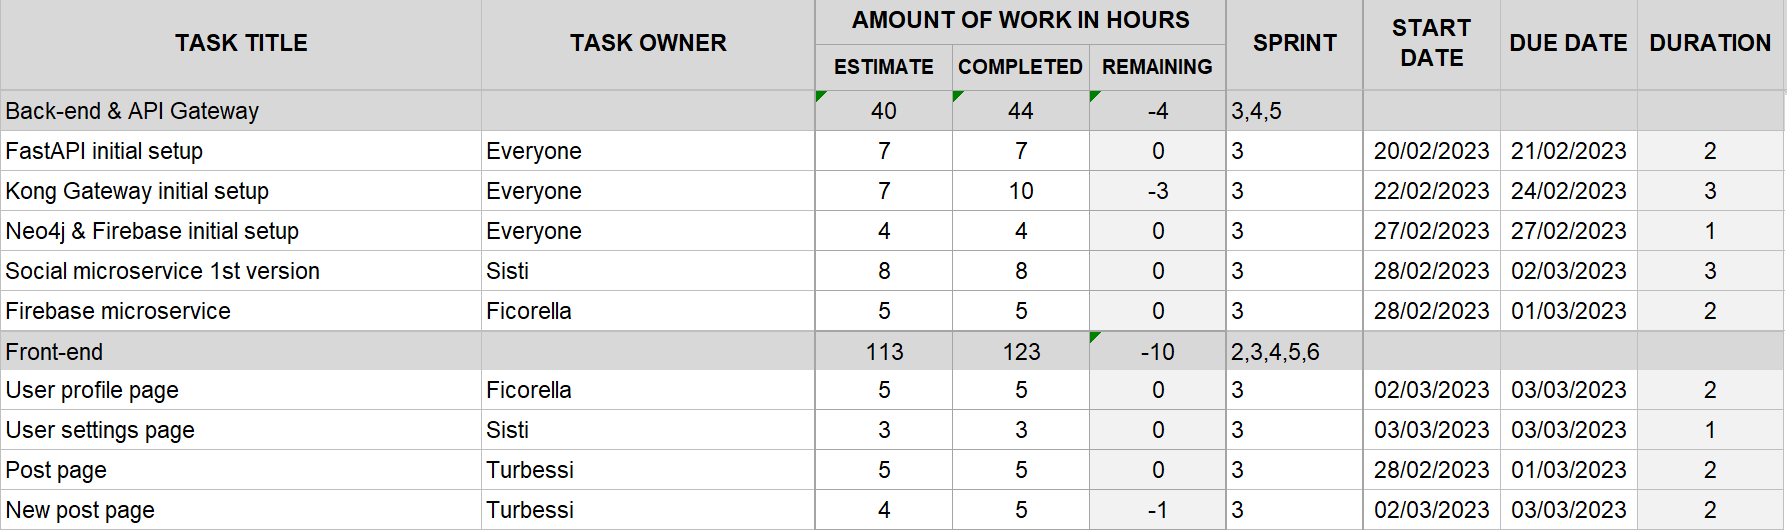
\includegraphics[width=1\textwidth]{images/sprint3.png}
\end{figure}
\subsection{Sprint 4: 06/03/2023 - 17/03/2023}
\begin{figure}[H]
    \centering
    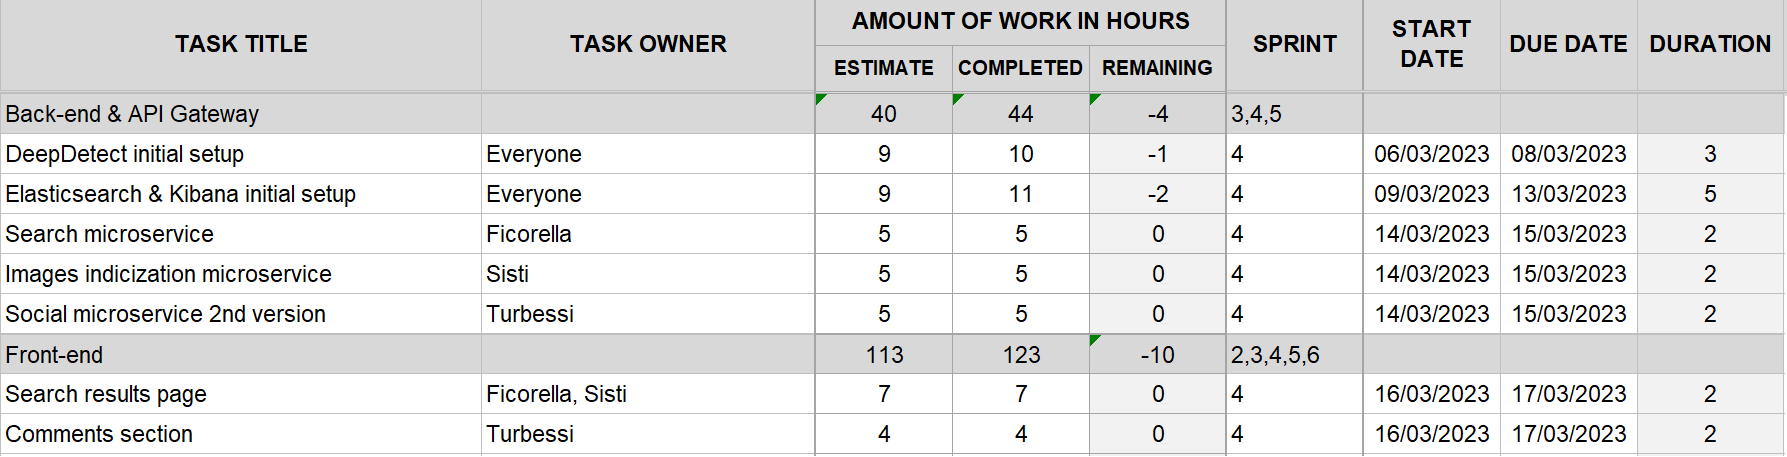
\includegraphics[width=1\textwidth]{images/sprint4.png}
\end{figure}
\subsection{Sprint 5: 20/03/2023 - 31/03/2023}
\begin{figure}[H]
    \centering
    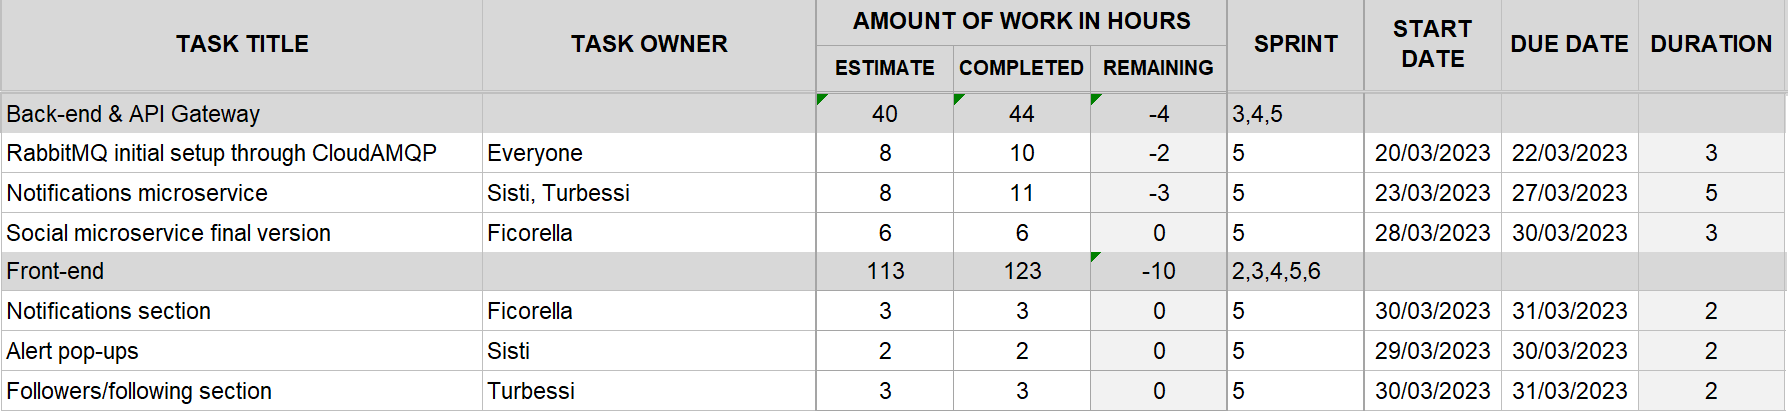
\includegraphics[width=1\textwidth]{images/sprint5.png}
\end{figure}
\subsection{Sprint 6: 03/04/2023 - 14/04/2023}
\begin{figure}[H]
    \centering
    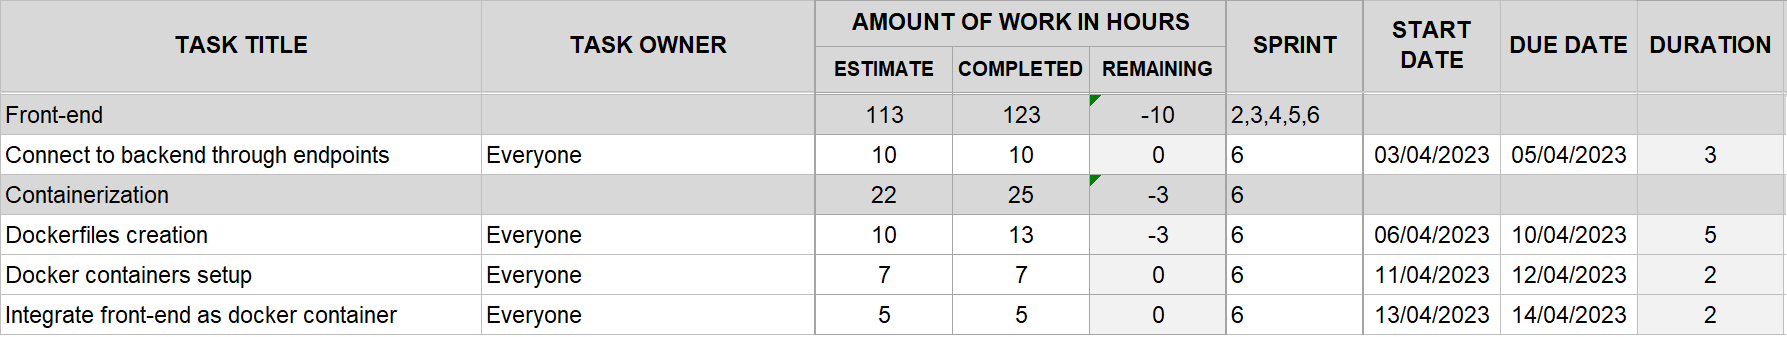
\includegraphics[width=1\textwidth]{images/sprint6.png}
\end{figure}

\newpage

\section{Burndown data}
\begin{figure}[H]
    \centering
    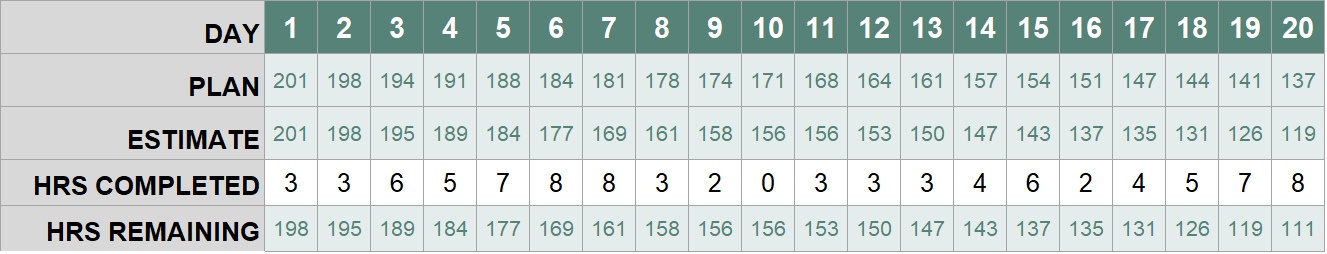
\includegraphics[width=1\textwidth]{images/burndown1.png}
\end{figure}
\begin{figure}[H]
    \centering
    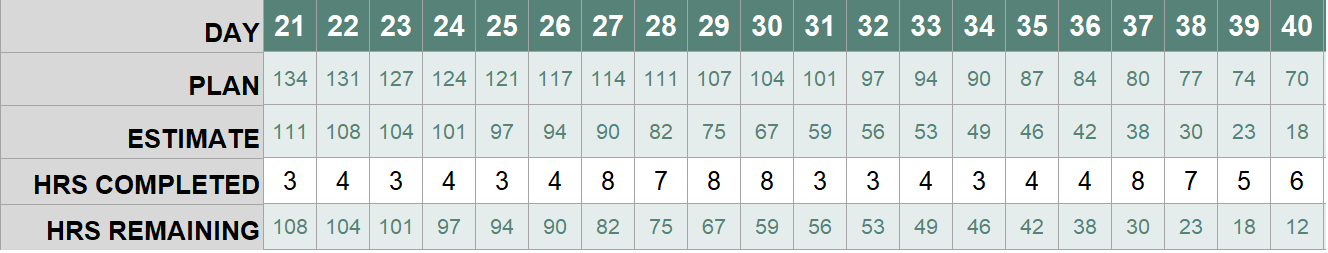
\includegraphics[width=1\textwidth]{images/burndown2.png}
\end{figure}
\begin{figure}[H]
    \centering
    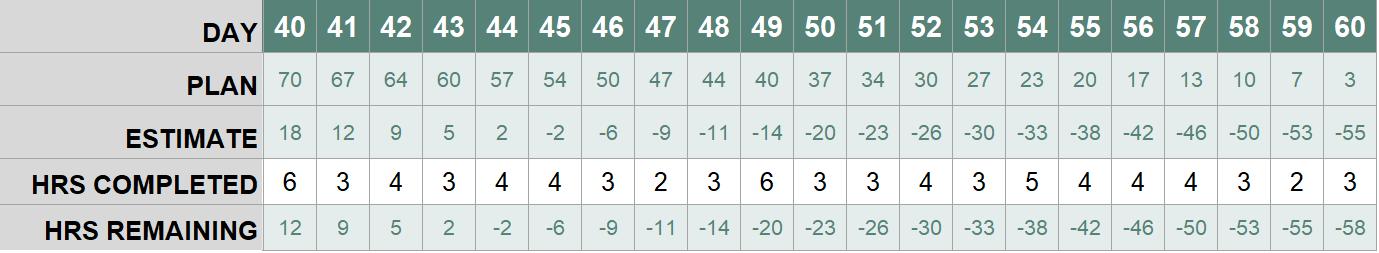
\includegraphics[width=1\textwidth]{images/burndown3.png}
\end{figure}
\begin{itemize}
    \item \textbf{Total estimated hours:} 201
    \item \textbf{Total completed hours:} 216
    \item \textbf{Total remaining hours:} -15
    \item \textbf{Total days:} 60
    \item \textbf{Average estimated hours per day:} 3.35
\end{itemize}

\newpage
\section{Burndown chart}
\begin{figure}[H]
    \centering
    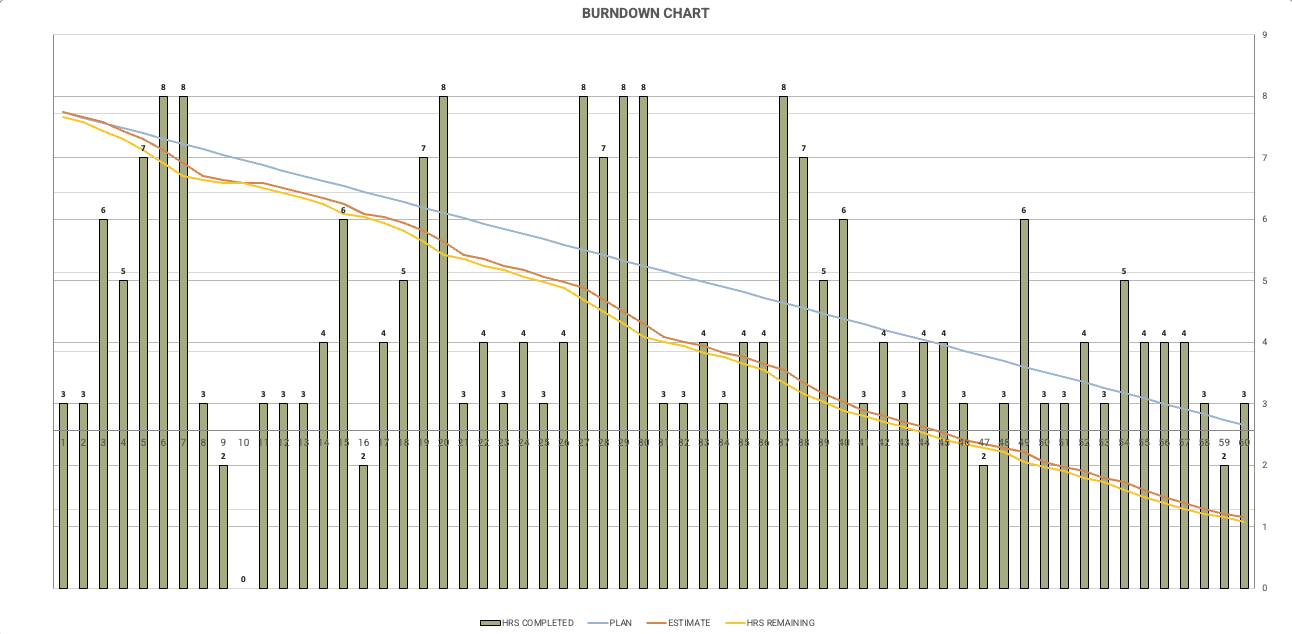
\includegraphics[width=1\textwidth]{images/burndownchart.png}
\end{figure}

\end{document}
